\chapter{Kinds without essences}
\label{ch:kinds-without-essences}

% TODO: Opening section introducing HPC from Boyd/biology goes here
% This section on discreteness follows that introduction.

\section{How clusters become discrete}
\label{sec:5:discreteness}

Here is the puzzle. Grammatical categories look discrete: a word is a noun or it isn't, a sentence is grammatical or it isn't. But the properties underlying those categories are continuous: frequency distributions shade smoothly from one pattern to another, phonetic realisations vary along continuous dimensions, semantic features don't come with sharp edges. How do discrete categories emerge from continuous substrates?

Two familiar answers, each half right. The essentialist says categories are discrete because their defining properties are discrete~-- either something has the essence or it doesn't. This gets the discreteness right but at the cost of definitions that don't exist. The prototype theorist accepts the gradience but can't explain the sharp edges or the stability~-- why don't categories blur into each other over time? We need a third option: an account of how mechanisms operating on continuous substrates produce categorical outcomes.

The answer lies in scale. A change that's negligible when you're far from a boundary becomes appreciable when you're close. That's why tolerance intuitions coexist with boundary intuitions~-- both are correct, just in different regimes. And the mechanisms that maintain categories~-- acquisition, entrenchment, alignment, transmission~-- are what keep the boundary where it is.

\subsection{The phase-transition intuition}
\label{subsec:5:phase-intuition}

Chapter~\ref{ch:what-we-havent-been-asking} introduced a physical analogy. Water has no essence of liquidity. The same H\textsubscript{2}O molecules constitute ice, liquid water, and steam. What differs is the collective behaviour: at certain temperatures and pressures, molecules settle into configurations we recognize as distinct phases. The boundaries between phases are real~-- you can skate on ice, swim in water, be scalded by steam~-- and they are sharp enough for practical purposes. But they are not maintained by essences. They are maintained by dynamics.

Phase transitions produce discreteness from continuous substrates. Temperature is continuous. Pressure is continuous. Molecular motion is continuous. Yet the macroscopic outcome~-- solid, liquid, gas~-- is categorical. The categories are real; they support predictions; they figure in explanations. And no essence is required.

This is suggestive. If physical systems can exhibit discrete, stable structure without essences, perhaps grammatical categories can too. But the analogy needs to be more than suggestive. We need to say precisely what it is about the dynamics that produces discreteness, and we need to show that something analogous operates in language.

The key insight from physics is that phase boundaries are \emph{scale-sensitive}. Near a phase boundary, small changes in temperature or pressure can flip the system from one phase to another. Far from the boundary, the same small changes have no categorical effect~-- the system remains solidly in one phase. The boundary is sharp, but its sharpness is a feature of the system at a particular scale of observation. Zoom in far enough and you find molecules fluctuating; zoom out and you find stable ice or stable water. The discreteness is real, but it emerges at the macroscopic level from continuous microscopic variation.

The same logic applies to vague predicates generally. Consider a heap of sand. Ten thousand grains is clearly a heap. One grain is clearly not. Somewhere between them lies a boundary. The boundary seems sharp~-- at some point, removing one more grain tips the collection from heap to non-heap. But we cannot identify where the boundary falls. Every attempt to specify a cutoff seems arbitrary. This is the Sorites paradox, and it has troubled philosophers for millennia.

The standard responses mirror those for grammatical categories. The epistemicist says the boundary is sharp but unknowable~-- there really is a precise number of grains where heaphood ends, we just can't find it. The degree theorist says heaphood comes in degrees~-- there's no sharp boundary, just a gradient from clearly-heap to clearly-not-heap. The supervaluationist says multiple precisifications are equally acceptable~-- the boundary is indeterminate, not because it's fuzzy, but because language doesn't fix a unique cutoff.

None of these quite captures the phase-transition intuition. The intuition says: the boundary is sharp (at the right scale), it is located in a determinate region (even if we can't specify it), and what maintains it is not an essence but a dynamic. The heap doesn't have an essence of heaphood; it has a configuration that, under the relevant conditions, clusters enough properties to count as a heap. Change the conditions enough and the clustering dissolves.

\subsection{Relative tolerance}
\label{subsec:5:relative-tolerance}

To make this precise, consider what \enquote{one grain doesn't matter} really means. It cannot mean that removing one grain \emph{never} makes a difference~-- that would entail that even a single grain is a heap. What it means is that removing one grain doesn't matter \emph{when you have many grains}. Ten thousand minus one is still clearly a heap. Fifty minus one might not be.

The difference is relative, not absolute. Removing one grain from ten thousand is a 0.01\% change. Removing one grain from fifty is a 2\% change. The same absolute change has different significance depending on the scale.

This suggests a principle:

\begin{quote}
\textbf{Relative Tolerance:} Changes that are negligibly small \emph{relative to the current scale} preserve category membership. Changes that are appreciable relative to the current scale may not.
\end{quote}

The principle is intuitive. When you're dealing with a clear heap~-- thousands of grains~-- removing one is negligible. When you're down to borderline cases~-- dozens of grains~-- removing one is appreciable. Tolerance holds in the first regime and fails in the second. The boundary lies where negligible changes accumulate into appreciable ones.

But \enquote{negligible} and \enquote{appreciable} are themselves vague. To make the principle precise, we need a framework that can handle the distinction rigorously. This is where nonstandard analysis helps.

\subsection{The hyperreal formalization}
\label{subsec:5:hyperreal}

The hyperreal numbers extend the real numbers to include \emph{infinitesimals}~-- quantities greater than zero but smaller than any positive real number \citep{Goldblatt1998LecturesHyperreals}. This might sound impossible, but the construction is mathematically rigorous; Abraham Robinson developed it in the 1960s. For our purposes, infinitesimals provide a way to make \enquote{negligibly small} precise without committing to any particular finite threshold. The application to vague predicates summarized here is developed fully in \citet{reynolds2025sorites}.

Here is how the framework applies to vague predicates. Let $P$ be a predicate like \textit{is a heap}, and let $\mu(x)$ be a measure of the relevant property~-- say, grain count. For successive cases $c_i$ and $c_{i+1}$ in a series, let $\Delta\mu_i = \mu(c_{i+1}) - \mu(c_i)$ be the change from one case to the next.

The Relative Tolerance principle becomes:

\begin{quote}
If $|\Delta\mu_i|/\mu(c_i)$ is infinitesimal, then $P(c_i) \leftrightarrow P(c_{i+1})$.
\end{quote}

In plain language: if the fractional change is infinitesimally small, the predicate's truth value is preserved. This captures the intuition that proportionally tiny changes don't matter, while allowing that accumulated changes can.

Now model the entire Sorites series~-- from clear heap to clear non-heap~-- as a \emph{hyperfinite chain} of $\omega$ steps, where $\omega$ is an infinite hypernatural number (Figure~\ref{fig:hyperfinite-chain}). This is a standard construction in nonstandard analysis: a sequence indexed by hypernaturals, behaving internally like a finite sequence but containing infinitely many elements from the external perspective.

\begin{figure}[t]
\centering
\includegraphics[width=0.85\textwidth]{figures/5.hyperfinite-chain.png}
\caption{The hyperfinite Sorites chain. The predicate $P$ (e.g., \emph{is a heap}) holds at every standard natural index: tolerance preserves truth across any finite portion of the series. The cutoff $K$ lies at a hypernatural index beyond all standard naturals~-- determinate within the model but not finitely specifiable.}
\label{fig:hyperfinite-chain}
\end{figure}

Within this hyperfinite chain, by the transfer principle of nonstandard analysis, any monotone sequence from $P$-true to $P$-false has a least index $K$ at which $P$ flips. This $K$ is a hypernatural~-- not a standard natural number, but a number in the extended system. And crucially, because we've stipulated that $P$ holds at all standard indices (encoding the intuition that tolerance holds throughout any finite portion of the series), $K$ must be nonstandard: infinitely large compared to any standard natural.

The picture that emerges:

\begin{itemize}
\item \textbf{Far from $K$}: The fractional change at each step is infinitesimal. Relative Tolerance applies. The predicate is preserved.
\item \textbf{Near $K$}: The fractional change is appreciable (no longer infinitesimal at this scale). Relative Tolerance is silent. The predicate can flip.
\item \textbf{At $K$}: The boundary. Sharp, determinate, located at a specific hypernatural index~-- but epistemically inaccessible because we cannot finitely specify which hypernatural.
\end{itemize}

This is why the Sorites induction fails. The inductive premise~-- \enquote{if $P(c_i)$ then $P(c_{i+1})$}~-- holds only where Relative Tolerance applies, which is far from the boundary. Near the boundary, the premise is false. The chain breaks not because tolerance is non-transitive, but because tolerance doesn't apply uniformly across the entire series.

\subsection{Sharp boundaries, fuzzy appearances}
\label{subsec:5:sharp-fuzzy}

The hyperreal model maintains classical bivalent logic throughout. At every index~-- including hypernatural indices~-- the predicate is either true or false. There are no degrees of heaphood, no fuzzy membership values. The boundary is sharp.

But the boundary is also inaccessible. It lies at a hypernatural index that we cannot specify using finite means. From our finite observational standpoint, we see clear heaps, clear non-heaps, and a region of uncertainty in between. The uncertainty is epistemic, not semantic: there is a fact of the matter about where the boundary falls; we just can't determine what it is.

The hyperreal view differs from epistemicism~-- Timothy Williamson's view that vague predicates have sharp boundaries, unknowable because of the limits of our discriminatory capacities \citep{williamson1994}. Both views say: sharp boundary, epistemic inaccessibility.

But the sources differ. For the epistemicist, the boundary is a brute metaphysical fact~-- fixed by the meaning of the word. For the hyperreal view, the boundary's existence is a consequence of the model's structure: the transfer principle plus monotonicity entail a cutoff at some hypernatural index. The sharpness falls out of the mathematics. The inaccessibility is built into what kind of thing a hypernatural index is. You can't finitely specify a nonstandard number any more than you can count to infinity.

This explains why tolerance intuitions and boundary intuitions can coexist. When you have a clear heap, you're right that one grain doesn't matter~-- the fractional change is negligible at that scale. When you're near the boundary, you're right that the situation is unclear~-- you're in the region where tolerance breaks down. Both intuitions are correct; they just apply to different regimes.

The model also explains why boundaries are stable. The boundary isn't an arbitrary stipulation imposed by speakers or analysts. It emerges from the structure of the hyperreal model, determined by the interplay between the tolerance principle and the monotonicity of the series. Different choices of nonstandard model (technically: different choices of ultrafilter in the construction) yield different specific values of $K$, but the structural features~-- sharp boundary, epistemic inaccessibility, scale-dependent tolerance~-- are invariant.

\subsection{From heaps to categories}
\label{subsec:5:heaps-to-categories}

Grammatical categories are not heaps. But they face the same discreteness problem. If the underlying properties~-- frequency, phonetic realization, semantic features, distributional patterns~-- vary continuously, how do discrete categories emerge?

The hyperreal framework extends naturally to this multi-dimensional case. The single dimension of grain count becomes a multi-dimensional feature space; the single predicate $P$ becomes a family of predicates $P_1, \ldots, P_n$ corresponding to different categories; and the linear Sorites series becomes a space of possible items, each located at some point in feature space.

The Relative Tolerance principle generalizes:

\begin{quote}
If $d(\mathbf{x}, \mathbf{x} + \Delta\mathbf{x}) / d(\mathbf{x}, \partial R_i)$ is infinitesimal, then $P_i(\mathbf{x}) \leftrightarrow P_i(\mathbf{x} + \Delta\mathbf{x})$.
\end{quote}

Here $\mathbf{x}$ is a point in feature space, $\Delta\mathbf{x}$ is a perturbation, $d$ is a metric on the space, and $d(\mathbf{x}, \partial R_i)$ is the distance from $\mathbf{x}$ to the boundary of category $i$'s region. In plain language: perturbations that are infinitesimally small relative to the distance to the nearest boundary preserve categorization.

\paragraph{The metric question.}
The notation $d(\cdot, \cdot)$ raises an immediate question: what metric? Grammatical features are heterogeneous. Some are ratio-scaled (frequency, duration). Some are ordinal (degree of acceptability). Some are binary (takes plural marking: yes/no). No single off-the-shelf metric applies to all.

The answer is that we don't need a unique privileged metric. What we need is a \emph{family of admissible metrics} that all induce the same small-change structure~-- the same notion of when a perturbation counts as negligible. Two metrics $d_1$ and $d_2$ are equivalent for our purposes if they are locally Lipschitz-equivalent in the region of interest: there exist positive constants $a, b$ such that $a \cdot d_1(\mathbf{x}, \mathbf{y}) \le d_2(\mathbf{x}, \mathbf{y}) \le b \cdot d_1(\mathbf{x}, \mathbf{y})$ whenever $\mathbf{x}$ and $\mathbf{y}$ are in the relevant portion of feature space. Metrics in the same equivalence class generate the same neighbourhoods of zero~-- the same judgments about which changes are infinitesimally small. Any member of that class suffices for the Relative Tolerance condition.

There is a principled way to construct such metrics for heterogeneous feature spaces. The strategy, familiar from statistical ecology and clustering analysis, proceeds in two steps \citep[cf.][]{gower1971}.

First, embed each feature into a dimensionless numerical scale:
\begin{itemize}
\item \textbf{Ratio and interval features} (frequency, duration, formant values) are standardized~-- divided by range or standard deviation~-- so that a unit change in one dimension is comparable to a unit change in another.
\item \textbf{Ordinal features} (ranked acceptability, degree of grammaticalization) are mapped to their rank position, rescaled to $[0,1]$.
\item \textbf{Binary features} (presence/absence of inflection, compatibility with a construction) are left as $\{0,1\}$.
\end{itemize}

After embedding, all coordinates are dimensionless and live in a common numerical space.

Second, place a weighted norm on the embedded vector:
\[
d(\mathbf{x}, \mathbf{y}) = \left( \sum_k w_k \left| \phi_k(\mathbf{x}) - \phi_k(\mathbf{y}) \right|^p \right)^{1/p}
\]
where $\phi_k$ is the embedding function for feature $k$, $w_k$ is a weight reflecting that feature's contribution to the homeostatic cluster, and $p = 1$ or $p = 2$. The weights can be estimated empirically (from regression coefficients, factor loadings, or feature-importance measures in classification tasks) or treated as parameters to vary in thought experiments.

The embedding is a heuristic, not a discovery procedure for Platonic dimensions. We don't expect factor analysis or MDS to reveal the true axes of grammatical space~-- there may be no unique decomposition. What we expect is that any adequate embedding will recover dimensions that are interpretable: dimensions that correlate with independently motivated grammatical or semantic scales. If a derived dimension tracks degree-modification compatibility, and degree-modification compatibility tracks the conceptual scale of gradability, then the embedding is doing its job.

This construction is a normed cousin of Gower distance, widely used for mixed-type data \citep{gower1971}, and it aligns with Gärdenfors's \emph{conceptual spaces}: multiple quality dimensions grouped into domains, each with its own metric, combined via weighted aggregation across domains \citep{gardenfors2000}. The connection to HPC is direct: the weights $w_k$ encode which properties play a stronger homeostatic role. Properties central to the cluster get large weights; free riders get small ones.

The point isn't that this construction is uniquely correct. The point is that a class of admissible metrics exists, all yielding the same small-change structure. The Relative Tolerance condition holds for all of them, not just one distinguished choice. Figure~\ref{fig:basin-visualization} illustrates the resulting landscape.

A clarification about dimensions. Some are conceptual in Gärdenfors's sense~-- grounded in perception and cognition, interpretable as quality scales that structure thought independently of any particular language. Eventivity, animacy, degree-scale structure: these show up in acquisition patterns, constrain semantic extension, have correlates in non-linguistic cognition.

Others are grammatical diagnostics: compatibility with plural morphology, occurrence in comparative constructions, position relative to the head. These may not correspond to conceptual dimensions at all. They're distributional reflexes of how a language happens to mark the underlying distinctions.

The feature space is therefore hybrid, combining conceptual geometry with grammatical symptomology. The HPC claim is that homeostatic mechanisms operate on both~-- that acquisition pressures and functional demands keep conceptual and grammatical dimensions aligned. Where they pull apart, the basin may shift or split. The geometry isn't pure cognition and it isn't pure grammar; it's the joint product of both.

English evidentiality offers a worked example. English has no grammaticalised evidential marking~-- no obligatory morphology indicating whether information is firsthand, reported, or inferred. But the conceptual dimension exists: speakers make evidential distinctions using lexical means (\mention{apparently}, \mention{reportedly}, \mention{I saw that}).

In languages with grammaticalised evidentiality~-- Tibetan, Turkish, many Amazonian languages~-- the grammatical and conceptual dimensions are aligned; the basin structure has both. In English, the conceptual dimension floats free of any grammatical basin. English speakers should show no clustering on evidential diagnostics, even though they make evidential distinctions conceptually. This is alignment failure without semantic loss. The concept persists; the grammatical basin doesn't form.

\paragraph{Visualizing the landscape.}
The three-dimensional surface we have been imagining is a visualization: the potential function $V$ is defined over the full feature space $X \subseteq \mathbb{R}^n$, with category cores corresponding to local minima and boundaries to the stable manifolds of saddle points. Any particular ``valley and ridge'' picture is the graph of $V$ over a low-dimensional slice of $X$ on which the relevant contrasts are visible. Choosing the metric~-- the weights $w_k$ and the embedding functions $\phi_k$~-- is, in effect, choosing a geometry for the energy landscape: which directions are steep, which are shallow, which features matter most for which basin. Relative Tolerance then says: stay within one valley when perturbations are small in that geometry.\footnote{The physics metaphor is heuristic, not literal. Potential minima correspond to prototypes (geometrical centres of categories); basins of attraction correspond to convex regions where similarity to the prototype dominates; \enquote{forces} are learning and update processes~-- acquisition, entrenchment, alignment~-- that shift representations toward or away from category centres. The metaphor earns its keep by unifying these phenomena under a single image; it doesn't commit us to actual energy functions computed by the brain.}

\begin{figure}[t]
\centering
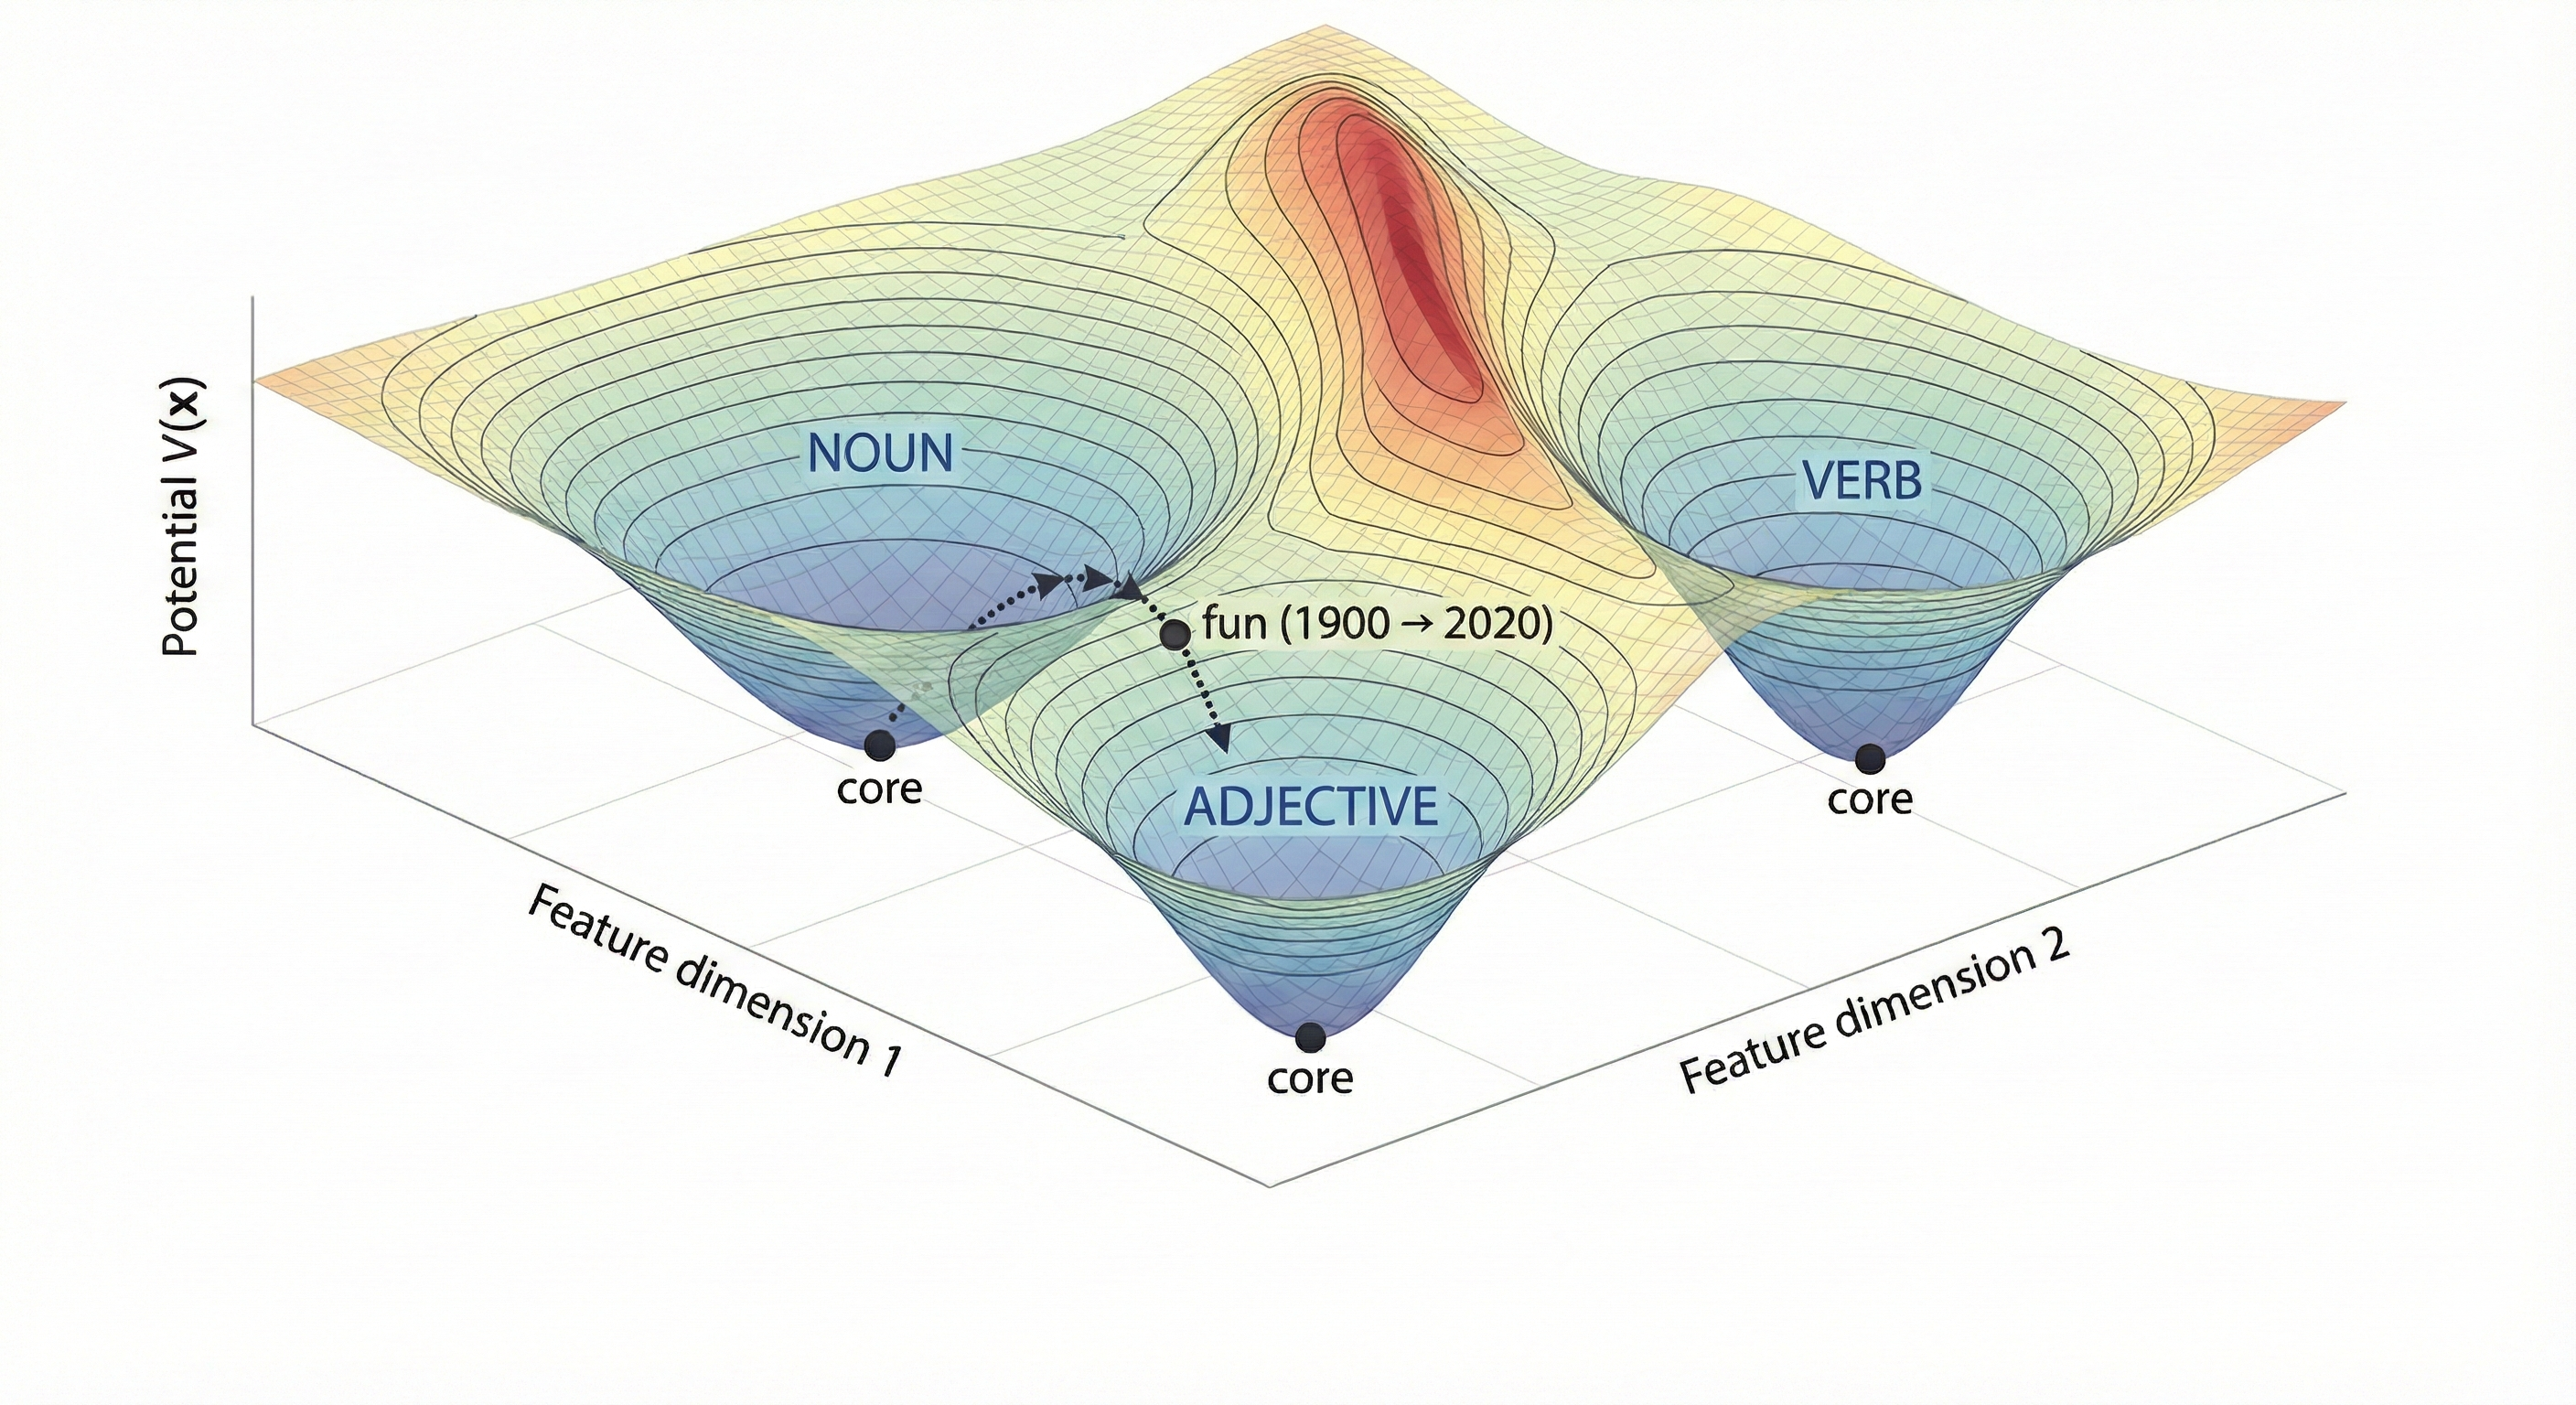
\includegraphics[width=\textwidth]{figures/5.three-basins.png}
\caption{A two-dimensional slice through grammatical feature space, with the potential function $V(\mathbf{x})$ plotted vertically. Category cores correspond to local minima; boundaries to ridges and saddle points. The noun and verb basins are separated by a high ridge (disjoint categories); the noun and adjective basins share a low saddle (porous boundary, overlapping membership possible). The trajectory of \emph{fun} illustrates diachronic movement from deep in the noun basin toward the noun--adjective boundary.}
\label{fig:basin-visualization}
\end{figure}

\paragraph{Basin structure.}
With a metric in hand, the multi-dimensional picture comes into focus. Each category occupies a region in feature space~-- a basin of attraction. Items deep in a basin are stably categorised: small perturbations don't move them out. Items near the boundary are unstable: the same perturbation that would be negligible elsewhere can flip the categorization.

The basins should be convex. If two items are stably categorised as nouns, items intermediate between them in feature space should be too. This is Gärdenfors's criterion for natural categories, and it holds here because the mechanisms maintaining the basin~-- entrenchment, analogy, transmission~-- operate by similarity. Items near the prototype pull their neighbours toward the same categorisation.

The potential-well metaphor captures this: a convex basin corresponds to a single local minimum, and gradient descent from anywhere in the basin leads to the same attractor.

The boundary cases that trouble essentialism~-- \mention{fun}, \mention{near}, \mention{otherwise}~-- are items near basin boundaries. They exhibit properties of multiple categories because they're in the region where tolerance breaks down. Their instability isn't noise; it's evidence about where the boundaries lie.

The categories remain discrete. At any point in feature space, an item is either in category $i$ or not. The boundaries are sharp, located at hyperreal distances that we cannot finitely specify. But the \emph{appearance} of gradience arises from epistemic limitations: we observe items at various distances from boundaries, and we cannot determine exactly where the boundaries fall.

\subsection{Mechanisms and basins}
\label{subsec:5:mechanisms-basins}

The hyperreal model describes the geometry of category boundaries. The HPC framework describes what maintains that geometry. The two are complementary.

Two stories, then. The first is representational: grammatical categories are regions in a feature space, with prototypes at centres and boundaries where similarity to multiple prototypes is balanced. This is the geometry.

The second is causal: the geometry persists because mechanisms~-- acquisition, entrenchment, alignment, transmission, functional pressure~-- exert forces that keep items clustered and boundaries stable. Conceptual-space approaches develop the first story in rich detail \citep{gardenfors2000,gardenfors2014}; HPC frameworks develop the second \citep{boyd1991,boyd1999}.

Both are needed. The geometry tells you what shape the categories have. The mechanisms tell you why they hold that shape.

Rosch's original insight remains intact: categories have graded structure organised around prototypes. What HPC adds is the causal story. \emph{Why} do prototypes attract? \emph{Why} does the category hold together across speakers and generations? The mechanisms~-- entrenchment, alignment, transmission~-- are the forces that maintain the prototype structure.

The hyperreal formalisation adds precision about boundaries: sharp but located at unreachable distances, exactly as tolerance intuitions suggest. Prototype theory describes the shape; HPC explains the stability; hyperreals explain the sharpness.

Consider what it takes for a basin structure to persist. The boundaries don't maintain themselves. Something has to keep items clustered in their basins; something has to resist drift toward boundaries; something has to stabilise the overall configuration. Without such forces, categories would dissolve: items would wander through feature space, boundaries would shift randomly, the discrete structure would blur into noise.

The homeostatic mechanisms are exactly these stabilising forces. They don't define the boundaries~-- that would be essentialism. They maintain the boundaries by exerting pressure on items in feature space.

\textbf{Acquisition} shapes the initial configuration. Children don't learn categories by being told definitions; they induce structure from input. The input reflects the existing basin structure~-- speakers produce items clustered in basins, with boundaries marked by distributional discontinuities. Learners who are sensitive to these patterns acquire the same basin structure, perpetuating it.

\textbf{Entrenchment} deepens the basins. High-frequency items are processed more automatically, stored with greater strength, and more resistant to analogical pressure. They anchor the category, providing stable reference points that other items cluster around. The more entrenched the central members, the steeper the basin walls, the more stable the category.

\textbf{Interactive alignment} maintains consistency across speakers. In conversation, speakers accommodate to each other's usage, converging on shared norms. This creates pressure toward uniformity within a speech community, keeping items in their basins even when individual variation would otherwise push them toward boundaries.

\textbf{Iterated transmission} filters variation across generations. Not all variants survive transmission; some are easier to learn, easier to produce, easier to understand. The variants that survive tend to be those well inside basins~-- clear exemplars, not boundary cases. Over generations, this filtering effect stabilizes the basin structure.

\textbf{Functional pressure} shapes the landscape. Categories exist because they serve functions: nouns package referents for tracking across discourse; verbs encode events and their participants; definiteness signals identifiability. Where functional pressure is strong, basins are deep and boundaries are sharp. Where it weakens, categories erode or restructure.

These mechanisms interact. Functional pressure determines which properties matter; acquisition determines how learners identify them; entrenchment determines which items anchor the category; alignment maintains community-level coherence; transmission filters what persists diachronically. The basin structure at any moment reflects the balance of all these forces.

The hyperreal model tells us what the basin structure looks like: sharp boundaries at hyperreal distances, tolerance holding within basins, instability near boundaries. The HPC framework tells us why the structure persists: mechanisms operating across multiple timescales, maintaining the clustering without defining it.

\subsection{Multi-category spaces}
\label{subsec:5:multi-category}

Linguistic categories don't exist in isolation. Nouns compete with verbs; adjectives shade into adverbs; prepositions overlap with both. The basin structure is not a set of independent regions but a tessellation of feature space, with categories abutting each other along shared boundaries.

This creates additional structure. An item near the noun-verb boundary might be stably a noun (because it's deep in the noun basin) or unstably categorized (because small changes could push it into the verb basin). The same item might be far from the noun-adjective boundary, so its nominal vs.\ adjectival status is never in doubt. Category membership is determinate in multiple dimensions simultaneously, with different degrees of stability in different directions.

Consider \mention{fun}. In the frequency-of-degree-modification dimension, it has drifted toward adjectives: \mention{very fun} is increasingly acceptable. In the takes-a-determiner dimension, it remains nominal: \mention{the fun we had} is unremarkable. The item sits near the noun-adjective boundary in one dimension, deep in noun territory in another. Its apparent mixed status reflects its location in a multi-dimensional space, not indeterminacy about what categories are. Figure~\ref{fig:diachronic-trajectory} traces this movement over time.\footnote{The trajectory sketched here is based on corpus evidence from COHA (Corpus of Historical American English) and Google Books Ngram data. Frequency of \mention{very fun} rises sharply after 1980; \mention{more fun} overtakes \mention{more amusing} in the 1990s.}

\begin{figure}[t]
\centering
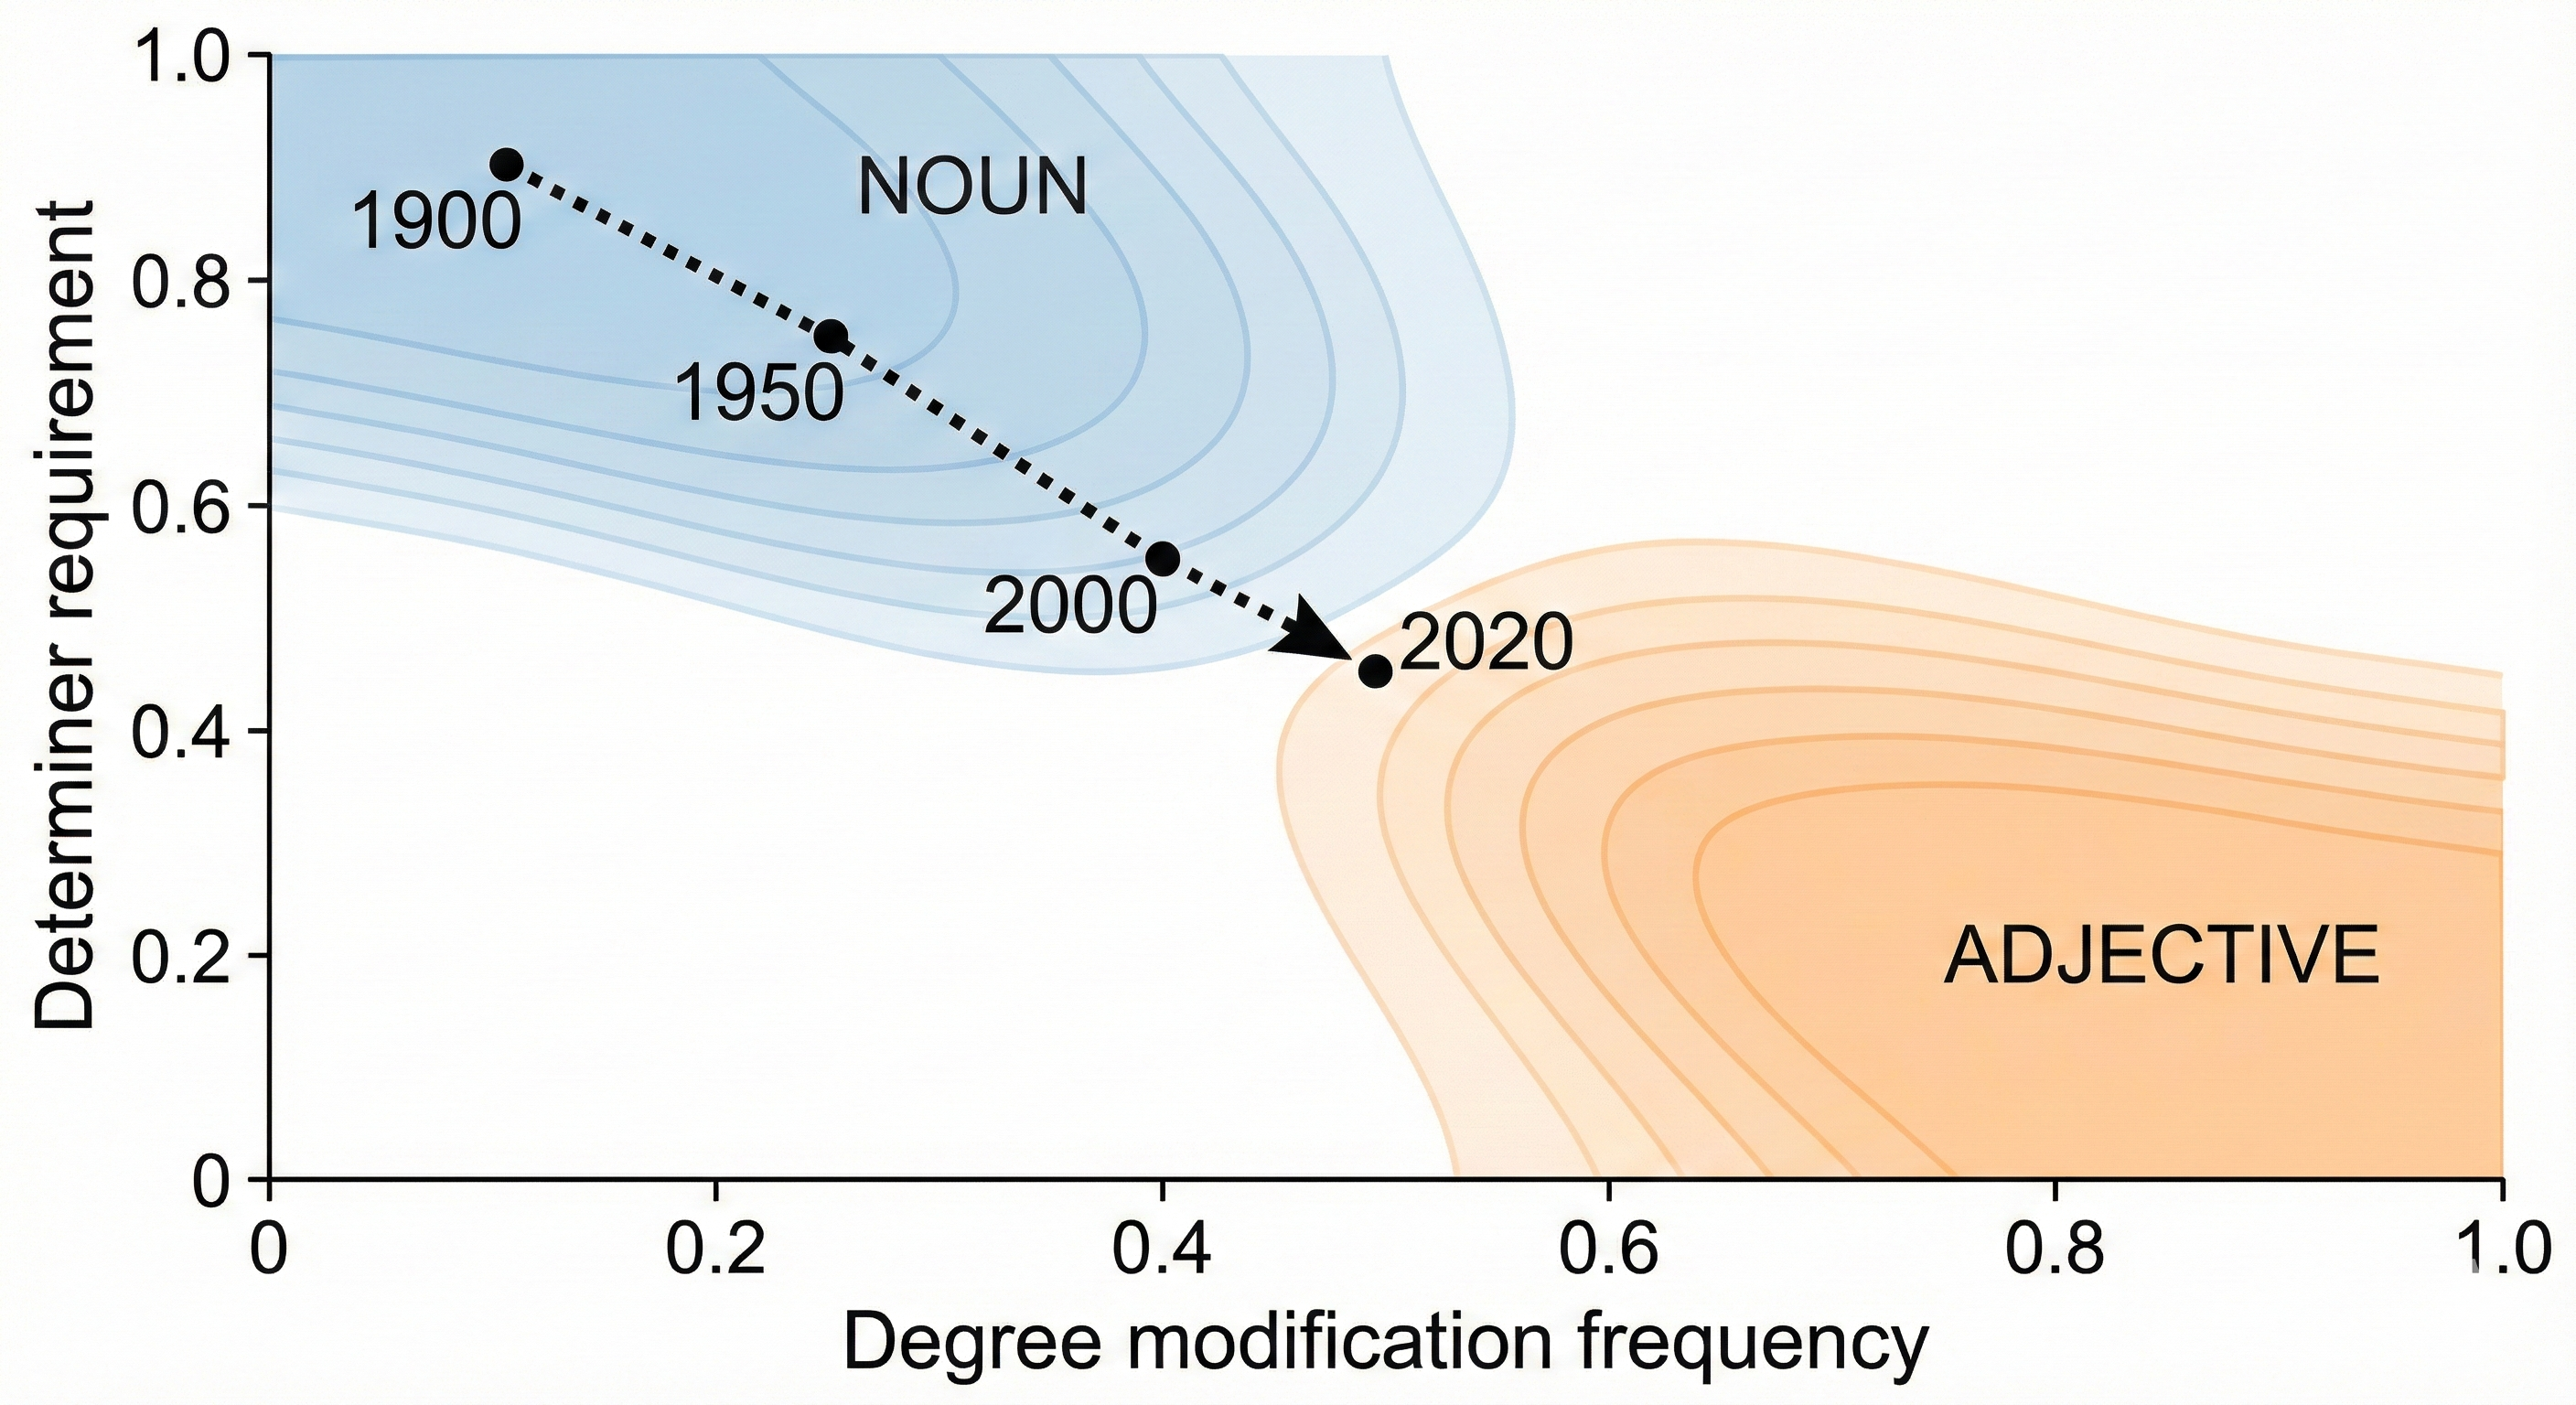
\includegraphics[width=0.85\textwidth]{figures/5.diachronic-trajectory.png}
\caption{The trajectory of \mention{fun} in a two-dimensional slice of feature space (degree modification frequency × determiner requirement). Dated points show corpus-estimated positions: from deep in the noun basin (1900) toward the noun--adjective boundary (2020). The contour shading indicates basin structure; the arrow indicates direction of diachronic movement.}
\label{fig:diachronic-trajectory}
\end{figure}

The same analysis applies to the existential debates about feature systems raised in Chapter~\ref{ch:what-we-havent-been-asking}. Is \textsc{gender} a natural kind, or is it reducible to \textsc{number}? The question becomes: do gender and number occupy distinct basins maintained by distinct mechanisms, or is gender a sub-region of a larger number basin, maintained by the same mechanisms at a finer grain?

If the mechanisms maintaining gender systems~-- agreement patterns, acquisition pathways, functional pressures toward nominal classification~-- are distinct from those maintaining number systems, then gender is a genuine natural kind: a separate basin in the space of grammatical features. If the mechanisms overlap substantially~-- if gender turns out to be number's machinery for individuation, as some theorists have argued~-- then the basins merge, and \textsc{gender} as a cross-linguistic category dissolves into \textsc{number}.

This is an empirical question, not a definitional one. The hyperreal model tells us what to look for: distinct basins with sharp boundaries and scale-dependent tolerance. The HPC framework tells us how to investigate: identify the mechanisms, trace their operation, determine whether they cluster distinct properties or the same properties at different scales.

Consider the Shilluk number system introduced in Chapter~\ref{ch:what-we-havent-been-asking}. English marks number with a suffix: \mention{cat}, \mention{cats}. Shilluk marks it through stem-internal changes in tone, vowel length, and voice quality~-- a singular/plural pair might differ only in whether the vowel is short, long, or overlong, or in whether the tone is Low or Fall. The exponence is lexicalised: each pair must be learned; no productive rule derives one from the other.

What does the HPC + hyperreal view say about this? Both English and Shilluk number systems occupy basins in a feature space whose dimensions include obligatoriness (number must be specified), agreement scope (specifier, verb, other constituents), and semantic function (individuation of entities). The exponence dimension~-- where English is affixal and Shilluk is fusional/suprasegmental~-- places them in different regions of morphophonological space but the same region of morphosyntactic and semantic space. They're in overlapping basins, not identical ones.

The mechanisms maintaining the two systems are partially shared (acquisition of obligatory contrast, iterated transmission of the singular/non-singular distinction) and partially distinct (rule-based productivity in English, lexical storage in Shilluk). The prediction is that where the mechanisms align~-- the functional pressure to distinguish singular from plural~-- the categories should pattern similarly across languages. Where they diverge~-- the phonological substance of the exponence~-- we should expect variation. That's exactly what we find. The basin boundary for \textsc{number} is sharp in both languages (a noun is singular or plural, not in between), but the basin's location in the full feature space differs, because different mechanisms weight different dimensions. The same analysis extends to noun-class systems like Swahili's, to Mandarin classifiers, to German gender. Wherever there's grammatical categorisation, there should be basin structure maintained by mechanisms.

A question arises: is the cross-linguistic similarity \emph{convergence} or \emph{homology}? In biology, convergence means similar phenotypes arising independently (the wings of bats and birds), while homology means similarity inherited from a common ancestor (the forelimbs of all mammals). For \textsc{number}, the answer is probably convergence: the functional pressure to distinguish singular from plural exists in any language with nominal reference, and different languages have evolved different morphological solutions. The mechanisms overlap not because of common ancestry but because of common function. For \textsc{noun} and \textsc{verb}, the answer might be different: if these categories reflect universal constraints on predication and reference, they may be homologous~-- inherited from whatever cognitive architecture makes human language possible. The framework should distinguish these cases, and the mechanistic analysis provides the tools: shared mechanisms suggest homology; parallel mechanisms suggest convergence.

One might ask: if the HPC analysis just confirms that English number and Shilluk number are both \textsc{number}, have we learned anything? Yes: the framework explains \emph{why} they deserve the same label~-- not definitional fiat, but overlapping mechanisms maintaining overlapping basins. And it makes predictions: if we found a putative \enquote{number} category maintained by entirely different mechanisms with no overlap in the functional dimension, the framework would say it's not the same kind~-- same label, different basin.

\subsection{Gradient judgments, discrete categories}
\label{subsec:5:gradient-discrete}

The discreteness problem has a close cousin: the gradient-judgment problem. Speakers' acceptability judgments are notoriously gradient. Asked to rate sentences on a 1--7 scale, they distribute across the range, with clear acceptability at the extremes and uncertainty in the middle. If categories are discrete, why are judgments gradient?

The hyperreal framework suggests an answer. Distinguish the category from its measurement.

\textbf{Grammaticality}~-- the property of conforming to the grammar~-- is discrete. A sentence either satisfies the constraints or it doesn't. The boundary between grammatical and ungrammatical is sharp, located at a hyperreal threshold in some underlying dimension (perhaps accumulated constraint violation, or distance from prototype, or processing cost).

\textbf{Acceptability}~-- the measured response in judgment tasks~-- reflects grammaticality filtered through noise. Processing difficulty, frequency effects, task demands, individual variation, and measurement error all intervene between the discrete category and the gradient response.

Not all of these factors work the same way. Random fluctuations~-- trial-to-trial variation in attention, incidental processing load, measurement noise~-- blur the signal without shifting it. But frequency effects and task demands can systematically shift the mapping from grammaticality to acceptability. A borderline construction may be judged more acceptable if it's high-frequency than if it's low-frequency, even when both are equally grammatical. Instructions emphasising naturalness may locate the boundary differently than instructions emphasising correctness. These are biases, not noise. The two-layer model accommodates them: different contexts may activate different effective basin configurations, shifting where tolerance breaks down.

This predicts:
\begin{itemize}
\item Clear cases cluster at scale extremes (1s and 7s), because items deep in the grammatical or ungrammatical basin are stably categorized and noise doesn't flip them.
\item Borderline cases distribute across the middle, because items near the boundary are sensitive to noise~-- small processing fluctuations can shift judgments in either direction.
\item The gradient spread is widest near the boundary, not because grammaticality is gradient, but because that's where the signal-to-noise ratio is lowest (see Figures~\ref{fig:two-layer-model} and~\ref{fig:judgment-variance}).
\end{itemize}

This is a testable prediction. If the two-layer model is right, items independently rated as near category boundaries should show higher variance in acceptability judgments than items rated as central. The prediction isn't that boundary items get middling ratings~-- that's compatible with gradient grammaticality~-- but that their ratings should be more variable across trials and subjects. The pattern should show up as a hyperbolic relationship between distance-to-boundary and judgment variance. Existing work on gradient acceptability already points in this direction: \citet{sprouse2013} found that judgment variability correlates with distance from prototypical (un)grammaticality, and \citet{dabrowska2010} showed systematic individual differences in judgments of complex constructions~-- exactly what you'd expect if different speakers have slightly different basin structures.

This last point deserves emphasis. The basin structure isn't uniform across speakers. Speakers with different input histories~-- more or less exposure to written registers, different dialectal backgrounds, varying levels of literacy~-- will have basins with different shapes and different boundary locations. The hyperreal model accommodates this naturally: each speaker's grammar is a different model, with a different boundary index $K$. What varies across speakers isn't just noise; it's the underlying geometry. The framework predicts that variability in judgments should be highest for constructions that fall near the boundary \emph{for most speakers}~-- and that speakers who agree on central cases may nonetheless diverge on peripheral ones, because their boundaries are located at different hyperreal indices.

\begin{figure}[t]
\centering
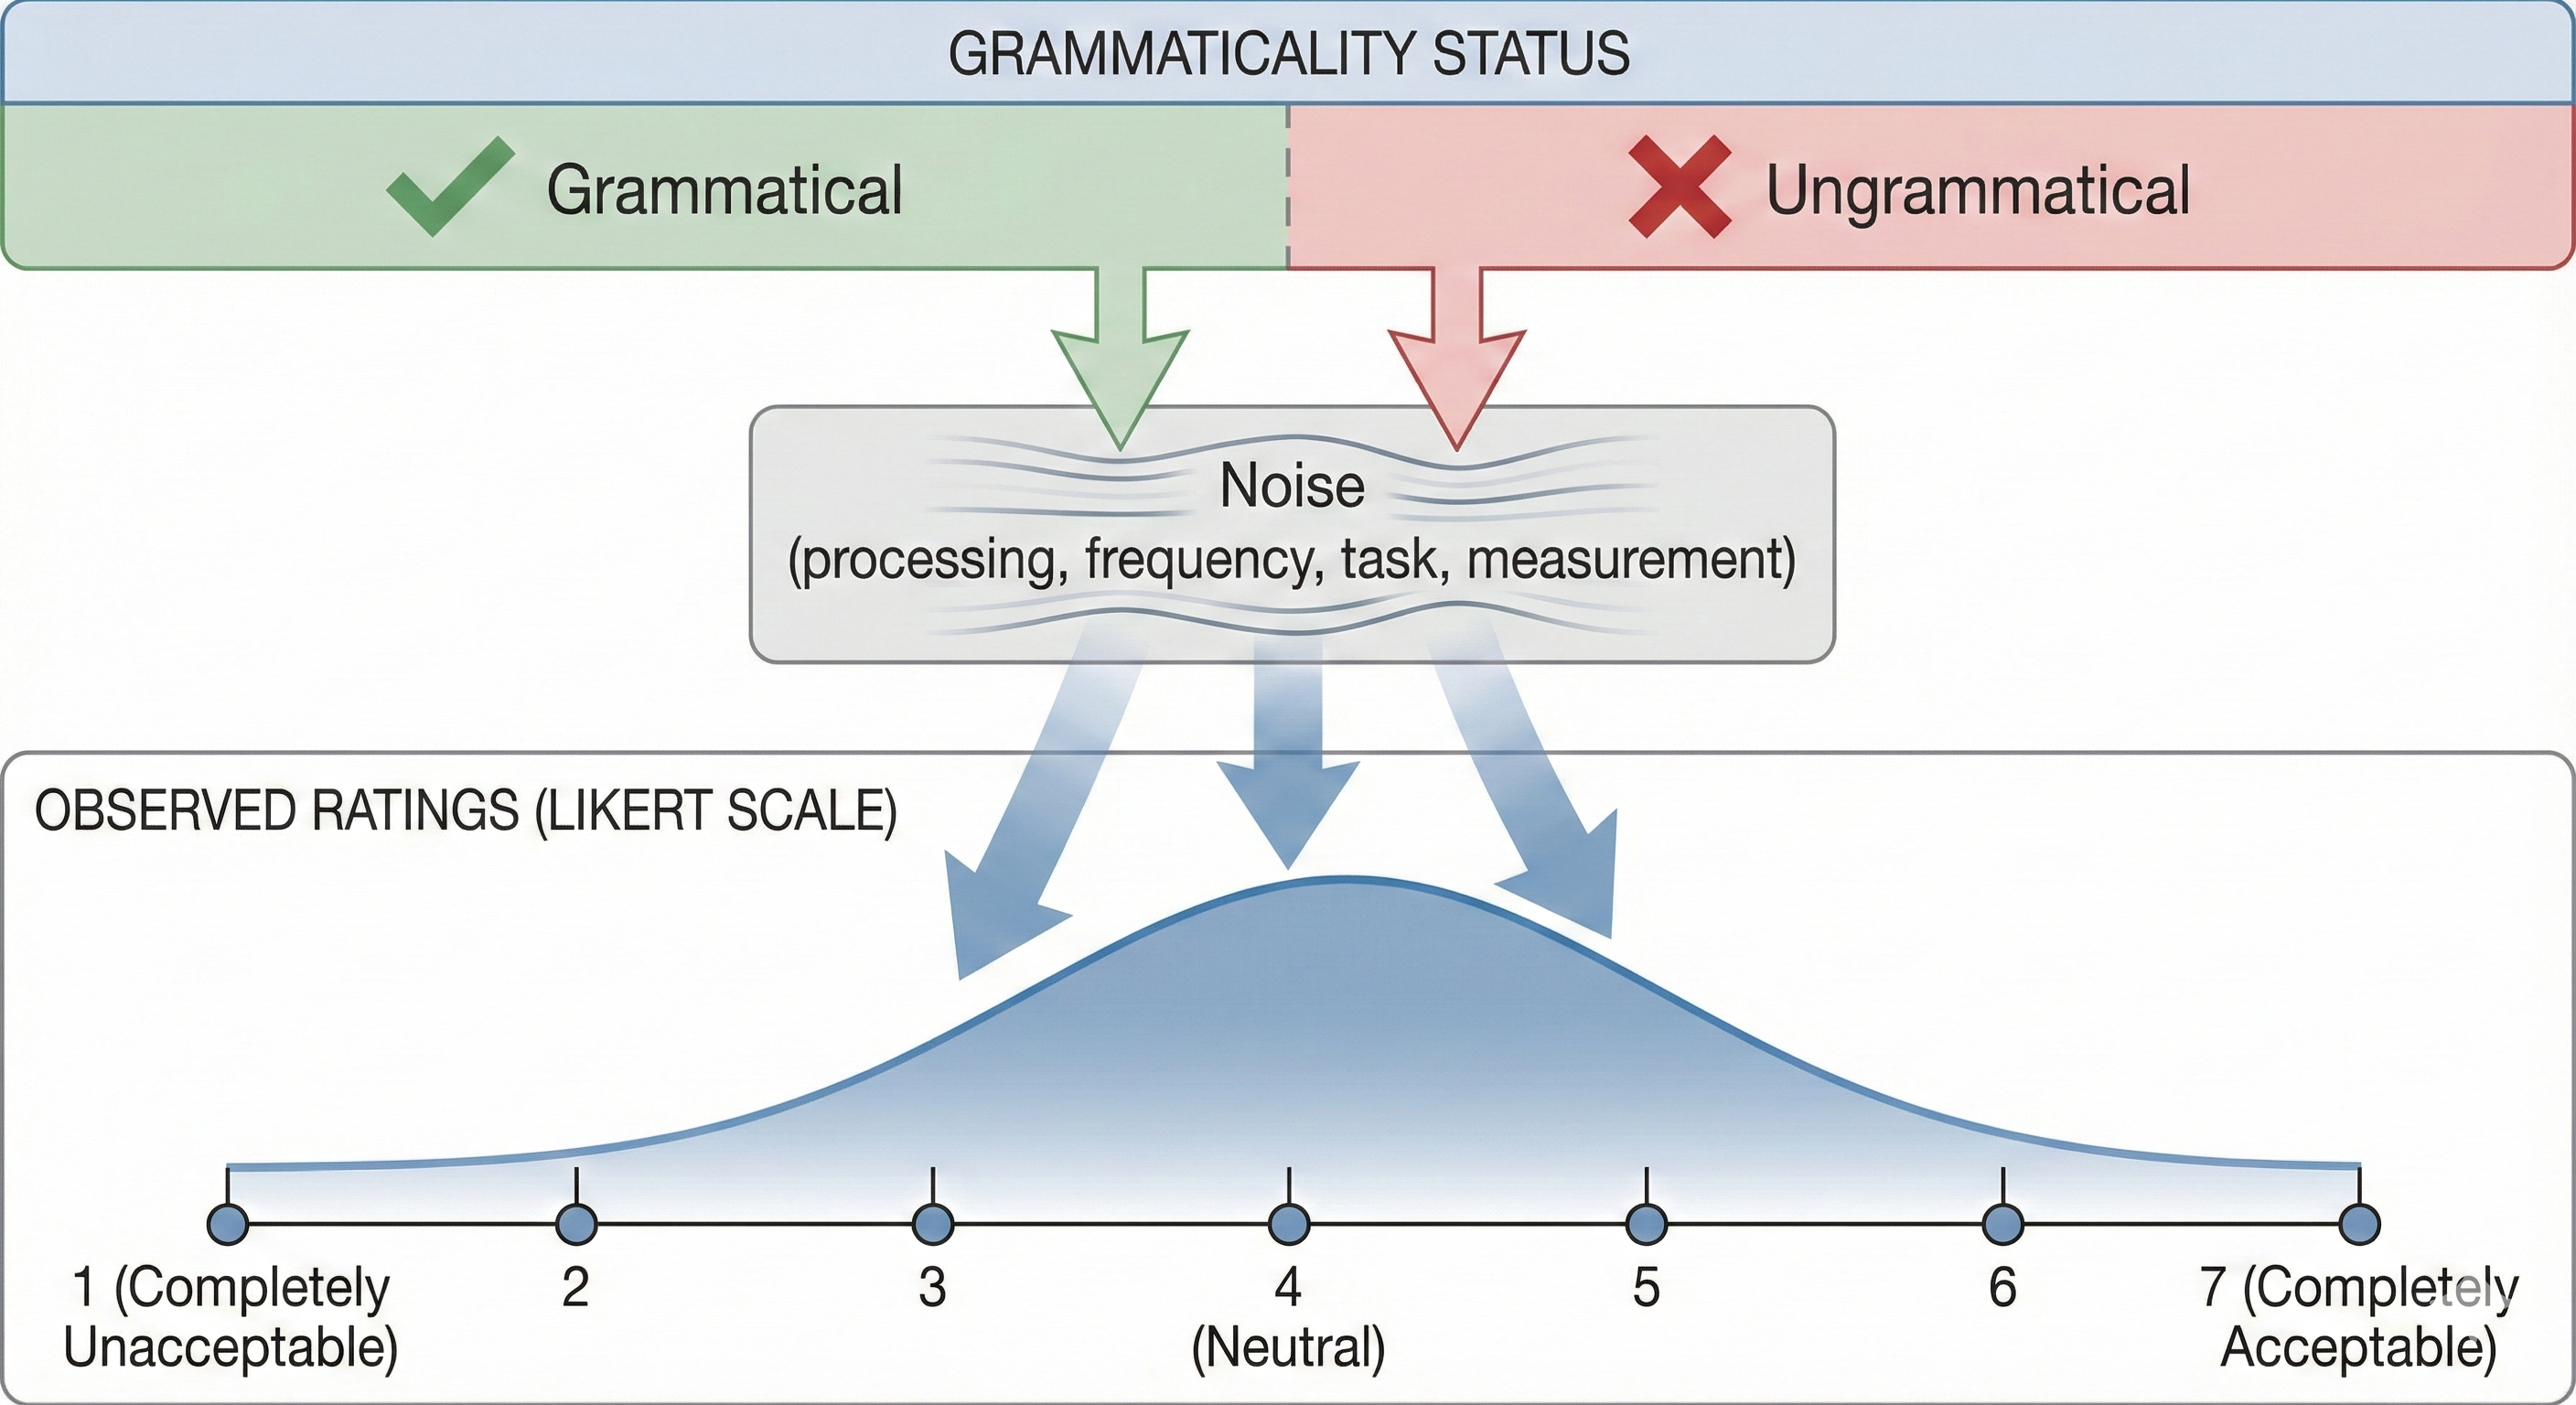
\includegraphics[width=0.85\textwidth]{figures/5.two-layer-grammaticality.png}
\caption{The two-layer model. Discrete grammaticality (binary: grammatical or ungrammatical) is filtered through processing and measurement noise to produce gradient acceptability judgments. Items deep in basins produce stable judgments at scale extremes; items near boundaries produce variable judgments distributed across the middle of the scale.}
\label{fig:two-layer-model}
\end{figure}

\begin{figure}[t]
\centering
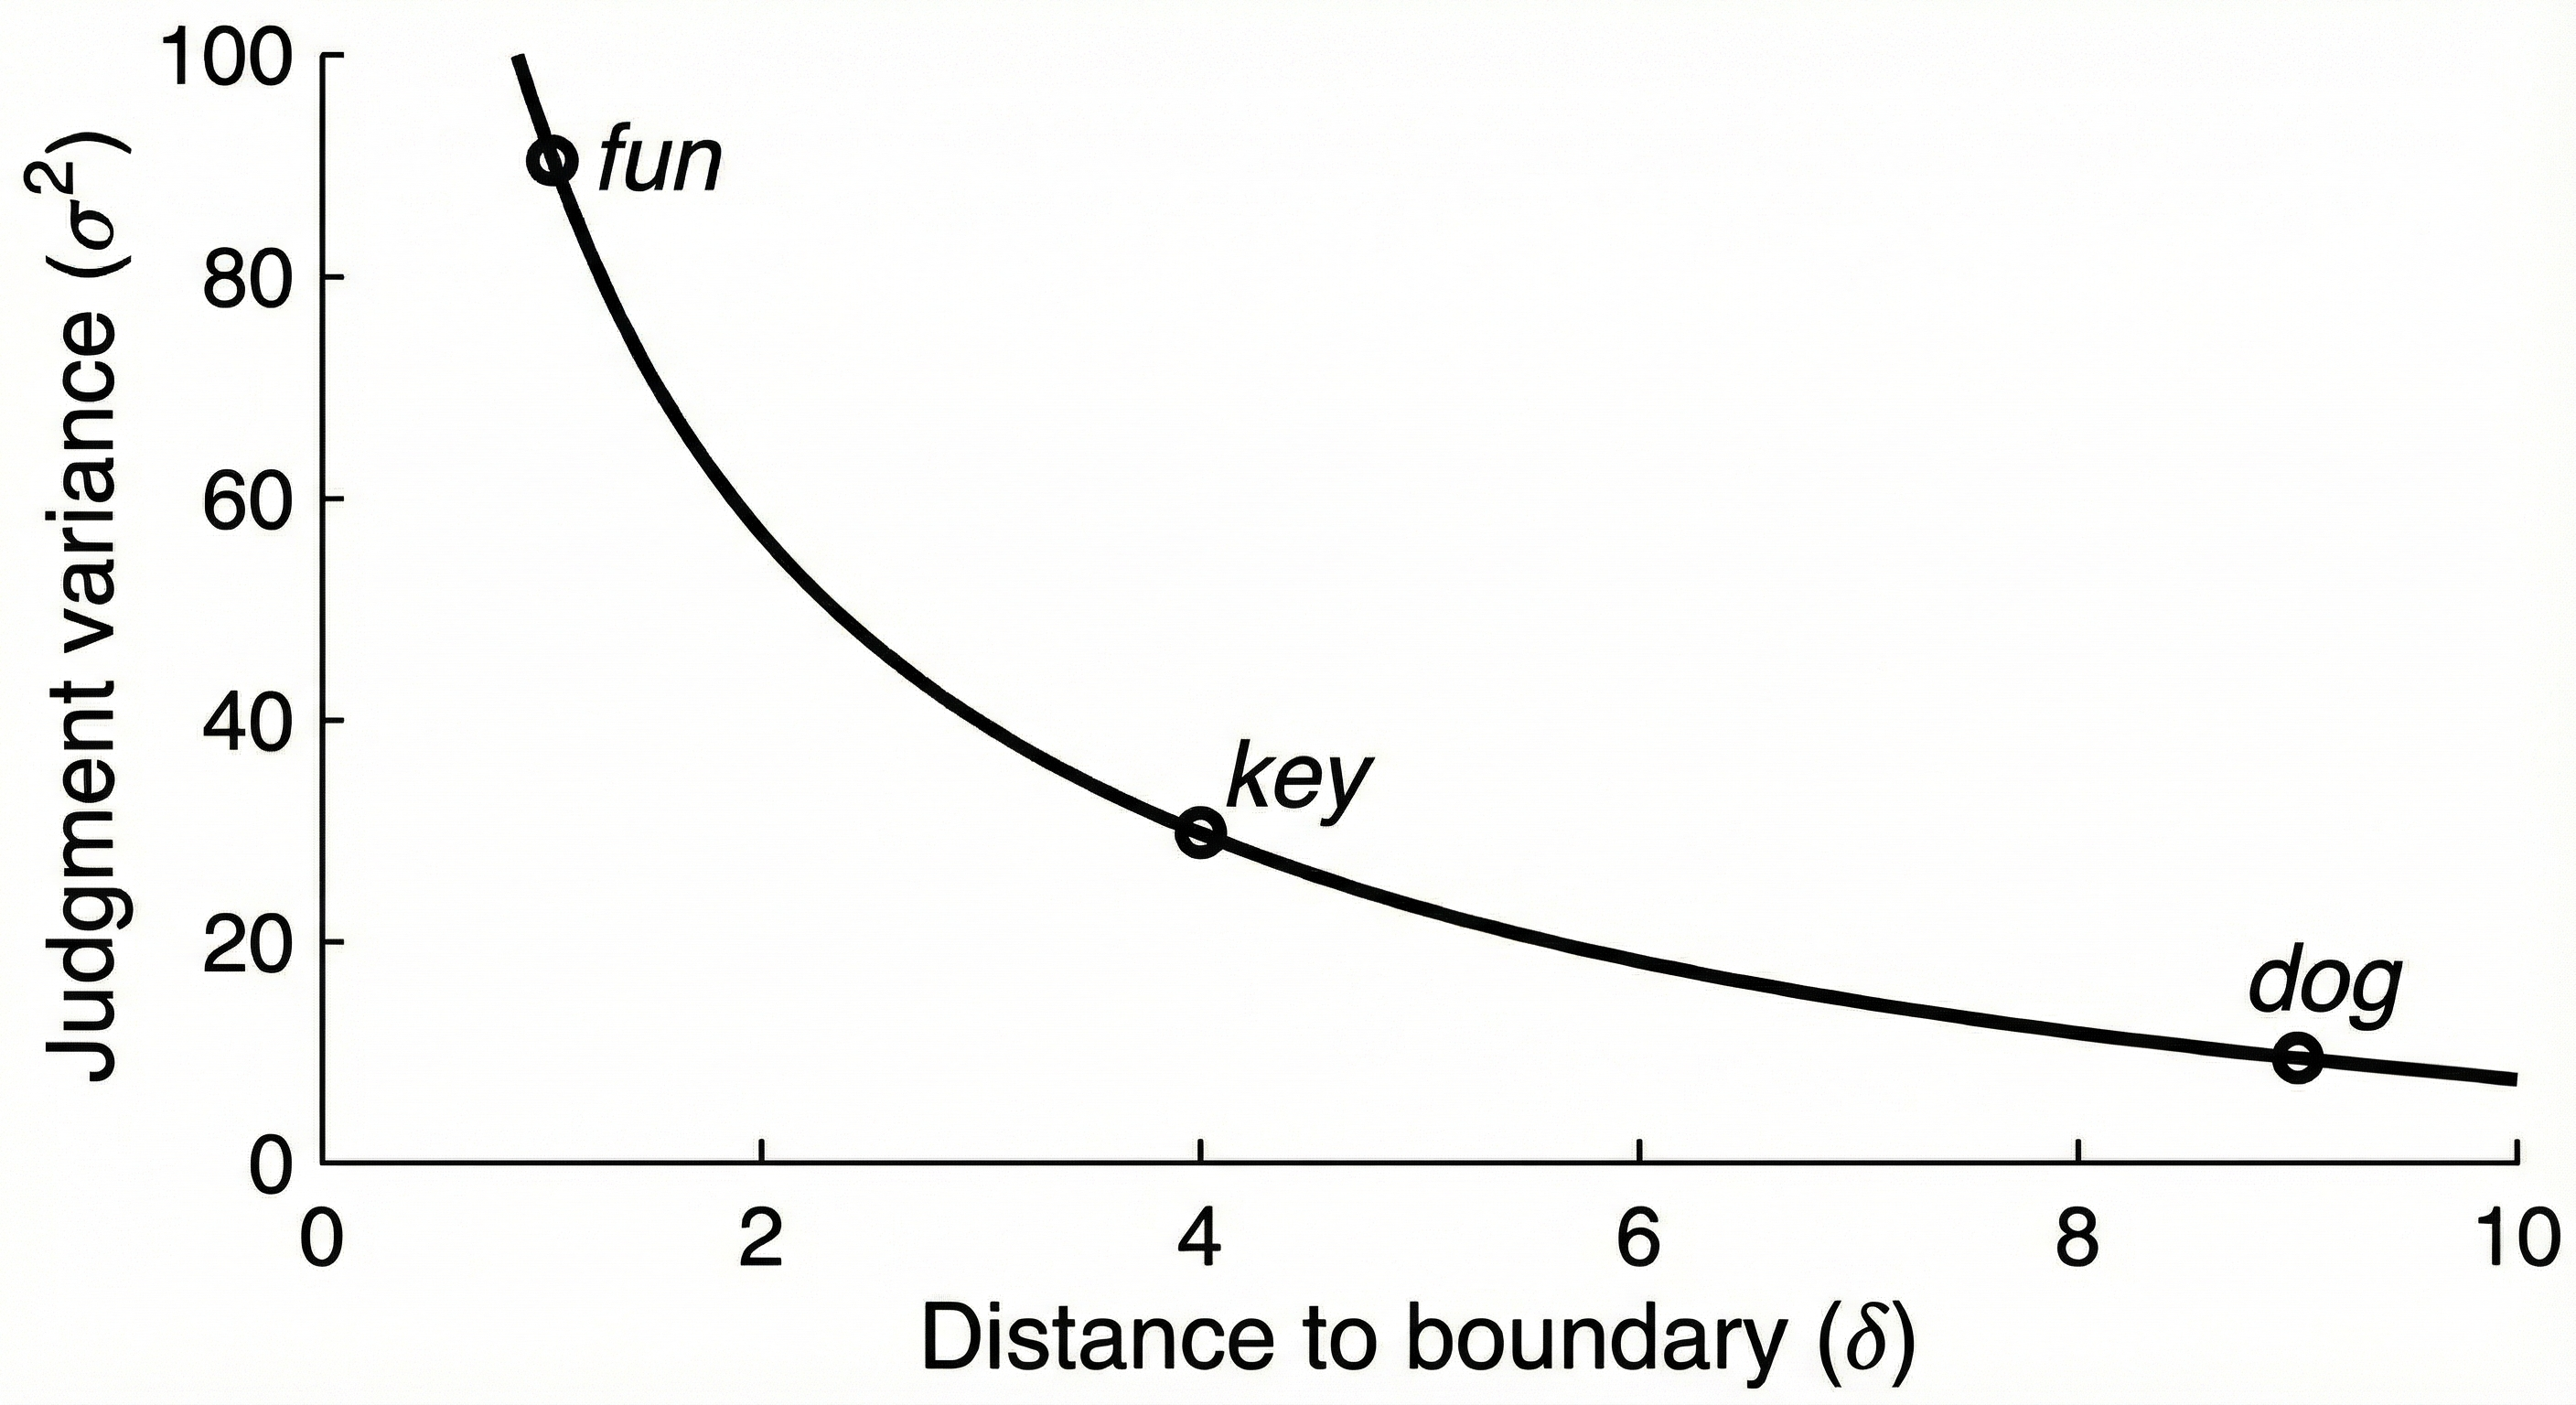
\includegraphics[width=0.85\textwidth]{figures/5.judgment-variance.png}
\caption{Predicted relationship between distance to category boundary and acceptability judgment variance. Items deep in basins (e.g., \mention{dog}) show stable judgments with low variance; items near boundaries (e.g., \mention{near}) show high variability. The hyperbolic relationship reflects the signal-to-noise ratio degrading as items approach the boundary.}
\label{fig:judgment-variance}
\end{figure}

This is not a new observation~-- the distinction between competence and performance has been with us since Chomsky. But the hyperreal framework adds precision. The boundary is not merely \enquote{somewhere in the grammar}; it's located at a specific (if unspecifiable) hyperreal threshold. The gradience is not merely \enquote{performance noise}; it's the predictable consequence of epistemic limitations near a sharp boundary.

Chapter~\ref{ch:grammaticality} develops this picture fully, arguing that grammaticality itself is a homeostatic property cluster~-- a category maintained by mechanisms, with a sharp boundary at hyperreal distance. For now, the point is that gradient judgments and discrete categories are compatible. The discreteness is in the structure; the gradience is in our access to it.

\subsection{Dual membership}
\label{subsec:5:dual-membership}

One puzzle remains. If categories are discrete~-- if at every point in feature space an item is either in or out~-- how can there be genuine dual membership? How can \mention{near} be both a preposition and an adjective, not contextually selected, not in transition, but stably both?

The answer is that discreteness holds predicate-by-predicate, not across predicates. The predicates \textit{is a preposition} and \textit{is an adjective} are each bivalent: at any point, each is either true or false. But they're not mutually exclusive. The basins can overlap.

This follows naturally from the HPC framework. Categories are maintained by mechanisms, not defined by partition. The mechanisms maintaining prepositionhood~-- patterns of complementation, head-of-PP status, lack of degree modification~-- are partially independent of those maintaining adjectivehood~-- gradability, predicative use, comparative morphology. An item can fall within the tolerance threshold for both, satisfying the clustering criteria for each.

Where the mechanisms align, the basins are disjoint: nouns and verbs occupy separate regions because the mechanisms that maintain them pull in different directions (Figure~\ref{fig:disjoint-overlap}, left). Where the mechanisms cross, the basins overlap: adjectives and prepositions share enough properties~-- predicative function, modification of nominals~-- that some items cluster with both (Figure~\ref{fig:disjoint-overlap}, right).

The regions of overlap are not arbitrary. They're located where the property clusters themselves overlap~-- where an item can satisfy the tolerance criteria for both categories simultaneously. These are exactly the cases that trouble essentialism: items that have \enquote{mixed} status because they satisfy criteria for multiple categories. On the HPC + hyperreal view, mixed status is not indeterminacy but dual location: the item is in two basins at once, stably, because the mechanisms that maintain each basin both apply.

\begin{figure}[t]
\centering
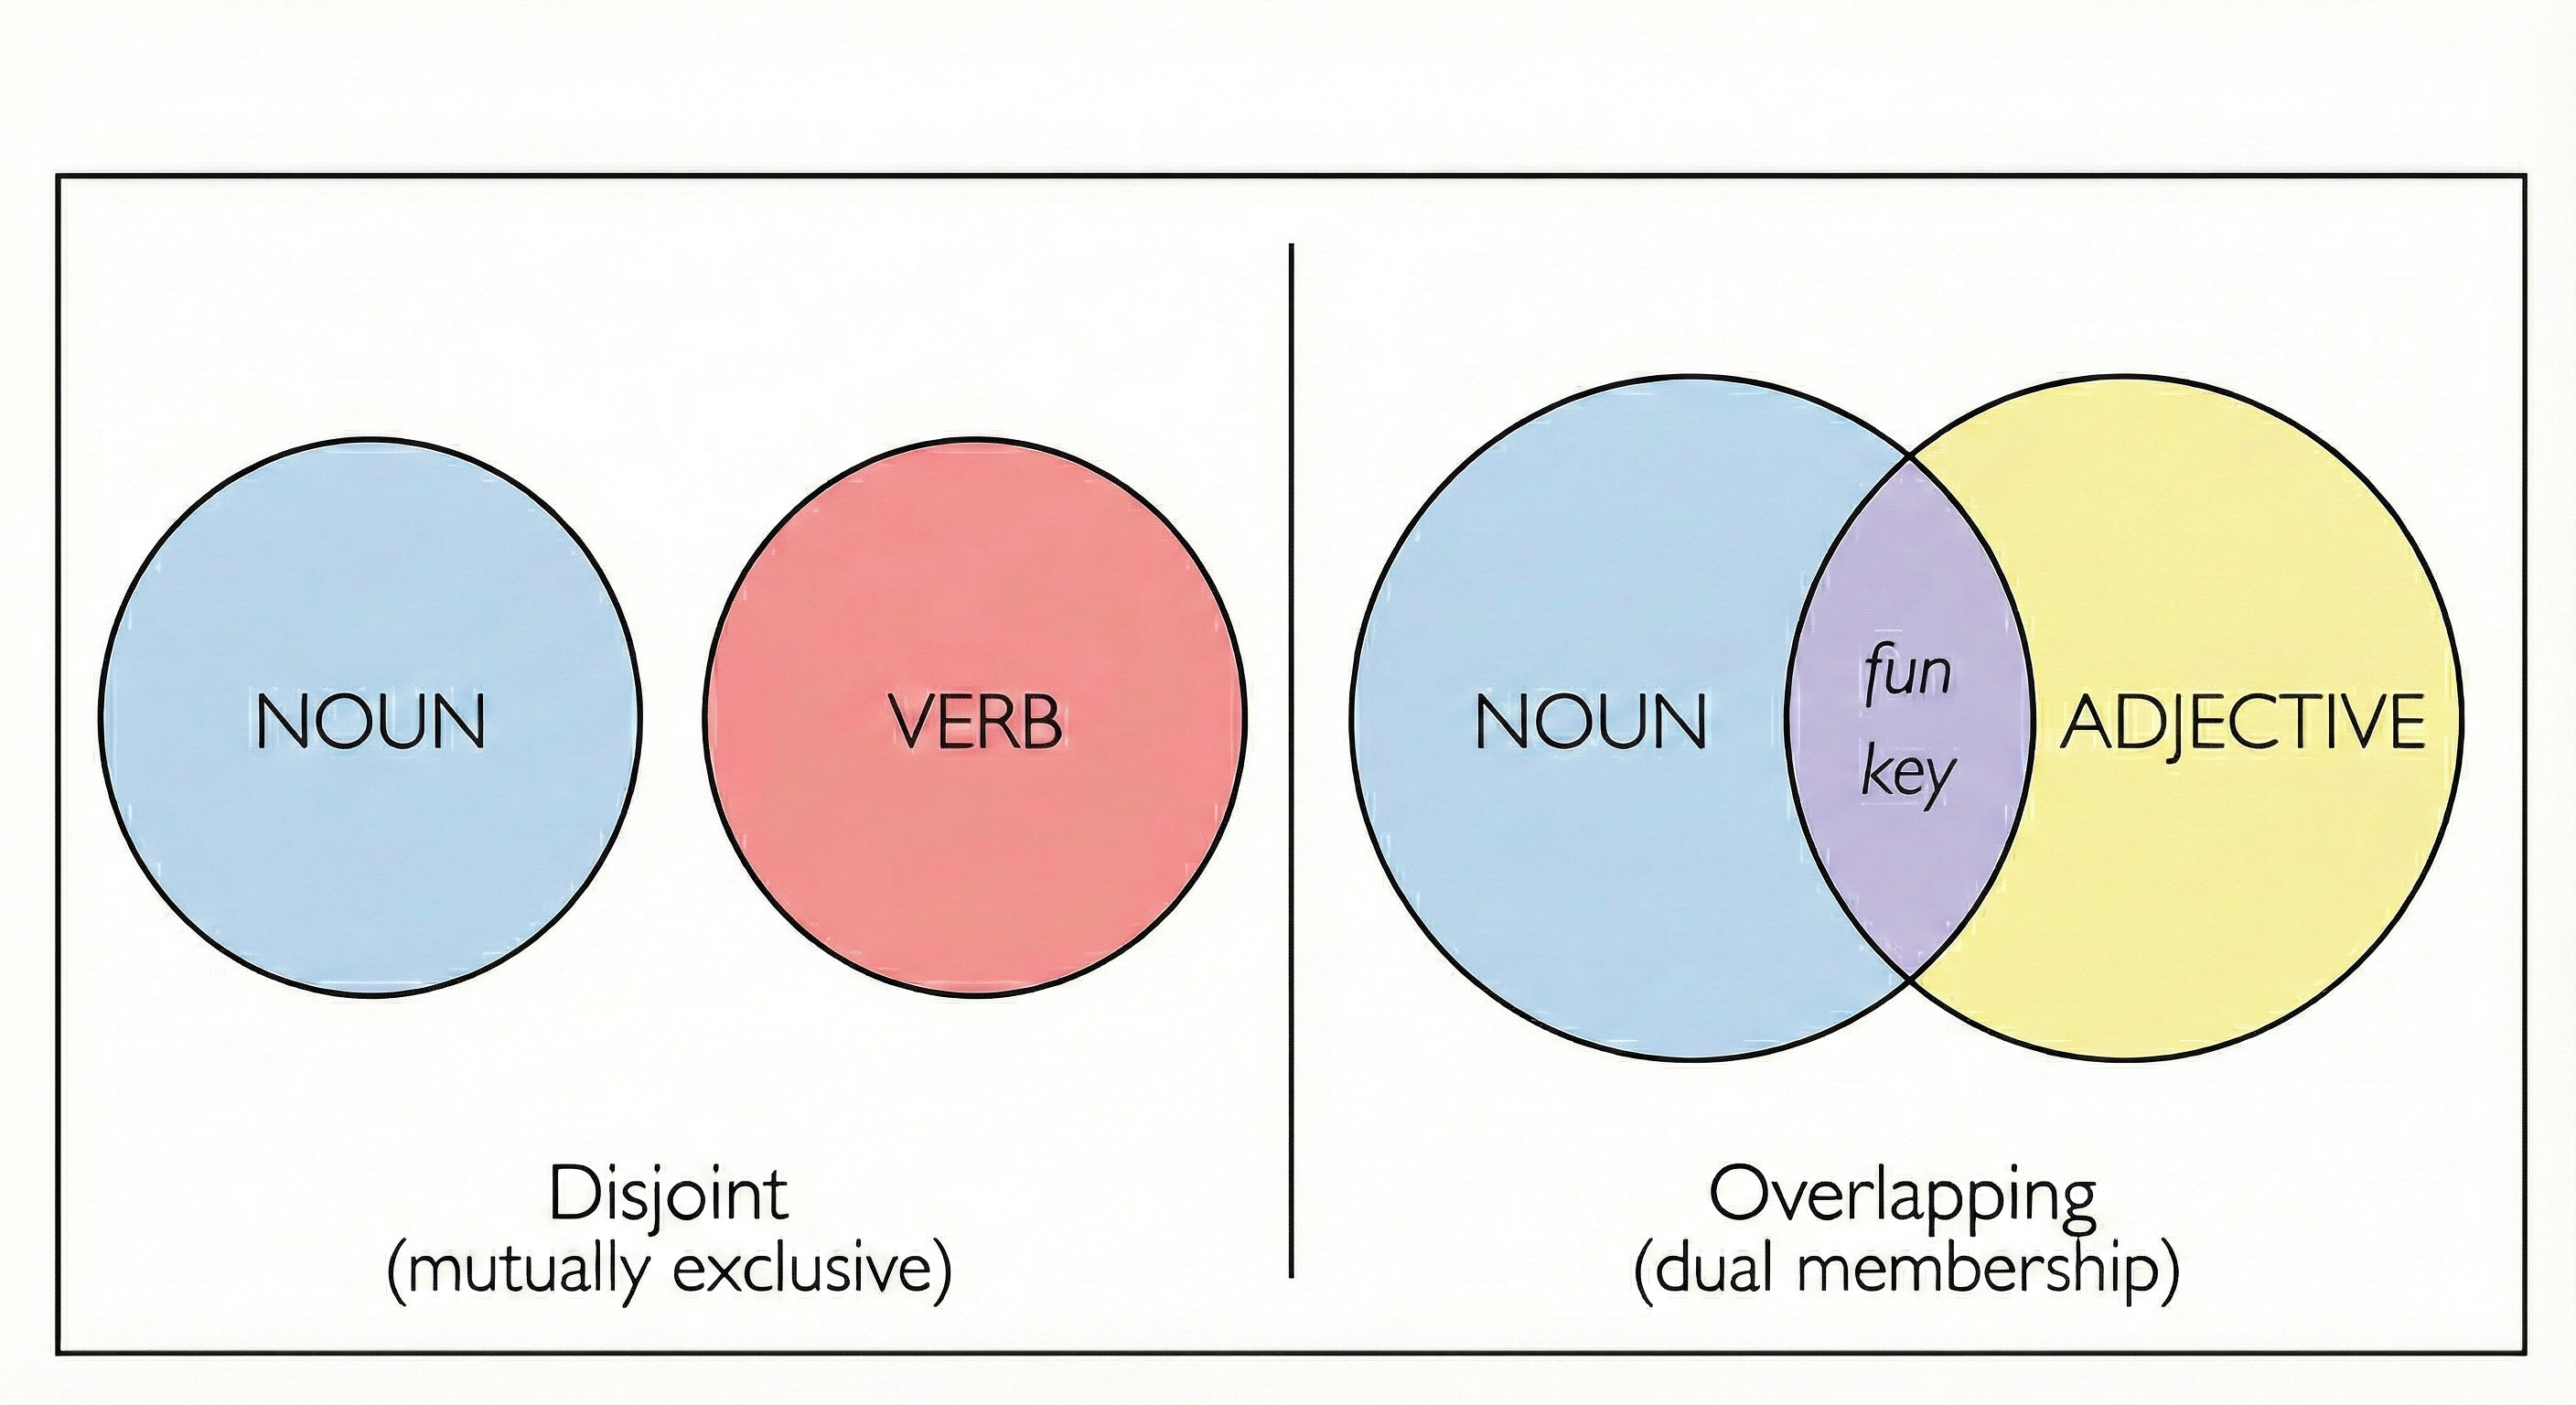
\includegraphics[width=0.85\textwidth]{figures/5.disjoint-overlap.png}
\caption{Disjoint vs.\ overlapping category basins. Left: noun--verb mechanisms pull in opposite directions, creating mutual exclusivity. Right: noun--adjective mechanisms are partially independent, permitting overlap. Items like \mention{fun} and \mention{near} occupy the overlap region, satisfying the clustering criteria for both categories simultaneously.}
\label{fig:disjoint-overlap}
\end{figure}

\subsection{Summary: discreteness without essence}
\label{subsec:5:discreteness-summary}

The discreteness problem asked: if underlying properties are continuous, how do discrete categories emerge?

The answer combines two components:

\textbf{Structure (hyperreal model):} Discrete boundaries arise from scale-dependent tolerance. Changes that are negligible at the current scale preserve categorization; changes that are appreciable can flip it. The boundary is sharp, located at a hyperreal threshold, epistemically inaccessible but structurally determinate.

\textbf{Maintenance (HPC framework):} The basin structure persists because mechanisms~-- acquisition, entrenchment, alignment, transmission, functional pressure~-- hold properties together. Without these mechanisms, categories would dissolve. With them, the clustering is stable even though boundaries are fuzzy at the edges.

Together, these explain how categories can be:
\begin{itemize}
\item \textbf{Real}: maintained by causal mechanisms, not merely stipulated.
\item \textbf{Discrete}: with sharp boundaries, not gradient membership.
\item \textbf{Fuzzy at the edges}: because tolerance fails near boundaries, producing instability and apparent gradience.
\item \textbf{Stable}: because mechanisms maintain the basin structure across time.
\item \textbf{Capable of change}: because mechanisms can shift, basins can migrate, boundaries can move.
\end{itemize}

This is what the essentialist wanted~-- real structure, sharp boundaries, determinacy~-- without what the essentialist thought was required: definitions, necessary and sufficient conditions, essences. The categories are real because they're maintained, not because they're defined. The boundaries are sharp because tolerance is scale-dependent, not because some property is binary. The determinacy is causal-structural, not definitional.

The nominalist was right that essences don't exist. The nominalist was wrong to conclude that determinacy fails. The HPC framework, formalized via hyperreal tolerance, shows how to have both: natural kinds without essences, discrete categories from continuous substrates, sharp boundaries that we cannot quite see.
